L'obiettivo del progetto è comprendere e mettere in atto metodi per la ricostruizione, o recupero, di 
immagini blurrate, lavorando su problemi test, ovvero generando immagini corrotte da un rumore 
Gaussiano applicandolo ad un set di immagini pulite in modo tale da analizzare il problema. 

Inizialmente verrà analizzata l'immagine \code{data.camera()} importata da
\code{skimage}, successivamente verranno analizzate 8 immagini con oggetti geometrici
 di colore uniforme su sfondo nero, realizzate da noi.

Il problema di deblur consiste nella ricostruzione di un immagine a partire da un dato acquisito
 mediante il seguente modello:
\[b=Ax+\eta\]
dove $b$ rappresenta l'immagine corrotta, $x$ l'immagine originale che vogliamo ricostruire, $A$ 
l'operatore che applica il blur Gaussiano ed $\eta$ il rumore additivo con distribuzione Gaussiana di
 media 0 e deviazione standard $\sigma$.

Per svolgere il progetto si farà uso dei moduli \code{numpy}, \code{skimage} e \code{matplotlib}
utilizzando il linguaggio Python.

Affinché risultino chiari i valori a cui andremo a riferirci nella relazione, bisogna tenere ben presente 
il significato di questi tre parametri. 

\textbf{PSNR (Peak Signal to Noise Ratio):} Misura la qualità di un immagine ricostruita rispetto all'immagine 
originale, la formula per calcolarlo è la seguente: \[PSNR = log_{10}(\frac{max\;x^\ast}{\sqrt{MSE}})\]

\textbf{MSE (Mean Squared Error):}  Con la sigla ci riferiamo all'errore quadratico medio ed è così ottenuto:
 \[MSE = \sqrt[2]{\frac{\sum_{i=1}^n\sum_{j=1}(x^{\ast}_{ij}-x_{ij})}{nm}}\]

I due valori sono inversamente proposizionali; più è alto il PSNR e basso l'MSE, più l'immagine sarà 
simile all'immagine originale. il PSNR dipende dall'MSE.

\textbf{Deviazione standard:} indica quanto sono distribuiti i dati rispetto alla loro media: 
un valore piccolo indica che i dati sono "ammassati" intorno al valore medio, 
mentre un valore grande indica che i dati sono distribuiti lungo tutto il grafico.

\begin{figure}[H]\centering
	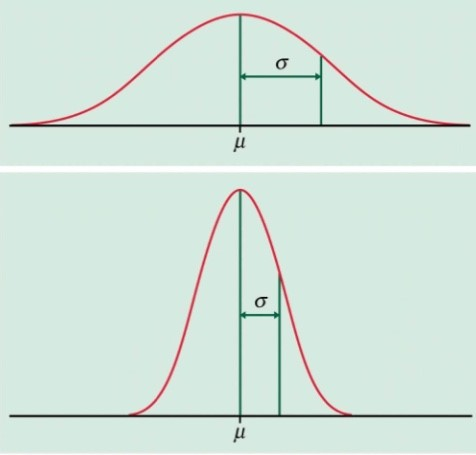
\includegraphics[width=0.3\textwidth]{MANCANTI/deviazione standard.jpg}
	\caption{Distrubuzione valori rispetto ad un valore medio}
\end{figure}